\documentclass{article}
\usepackage[utf8]{inputenc}
\usepackage{graphicx}
\usepackage[style=ieee]{biblatex}
\usepackage{multicol}
\usepackage{fullpage}

\addbibresource{outline_citations2.bib}

\title{APM348H Final Paper Outline}
\author{Agathe Yvinec Tolmer, Thomas Rimbot, Pranav Sadana }
\date{March 2020}

\begin{document}

\maketitle

\section{Introduction}
\quad The Iberian lynx, \emph{Lynx pardinus}, is the most endangered feline species in the world. It is found in Spain and Portugal and 20 years ago, its population was as small as 100 adult individuals in total. This was partly due to the main prey of the Iberian lynx, the European rabbit, \emph{Oryctolagus cuniculus}. During the second half of the 20th century, the European rabbit suffered from diseases like rabbit haemorrhagic disease which contributed to its decline. Since then, the remaining lynx populations have been protected and some individuals were reintroduced, leading to a total of 475 Iberian lynxes in 2017\cite{noauthor_iberian_nodate}.

\quad The Iberian lynx is also known to compete with cats (\emph{Felis sp.}) for preys and cats killed by lynxes are frequently reported. In 2007, an epidemic of Feline Leukemia Virus (FeLV) struck one of the populations of Iberian lynxes in Doñana, Spain. Out of approximately 50 lynxes, 12 got infected and 7 died within a year\cite{meli_feline_2010}. The virus was contracted by contact with infected cats, and then likely spread inside the lynx population. Furthermore, in 2017, conservation researchers monitoring the Iberian lynx population came across the first case of a lynx consuming a cat\cite{najera_lynx_2019}. Since cats also consume European rabbits, our 3 animals are linked by a trophic web of the shape Predator (lynx) – Mesopredator (cat) – Prey (rabbit). 

\quad In this paper, we aim to evaluate the spread of FeLV from cats to Lynxes with the help of compartmental SIR model coupled with a Lotka-Volterra population model. Since the virus appears to be more virulent in Lynxes, we aim to explore  the role played by cats as a reservoir of the virus using a sensitivity analysis on the contact and transmission rates. We investigate whether the cats spread FeLV to the Lynx or FeLV spreads within the lynx population. Further, we aim to model the population dynamics of the system to propose some conservation strategies to maintain the population of Lynx. 

\section{Model and Study system}
\quad Our project will mostly rely on two mathematical models: the Lotka-Volterra model for predator-prey dynamics and the SIR model for disease dynamics. The first will be expanded to take into account the presence of mesopredator (cats) so that we have a predator-mesopredator-prey dynamics. Then, we incorporate the SIR model into this new model and use it to simulate the spread of the disease. This approach will give us a set of differential equations that give us at each time the populations of lynxes, cats and rabbits, based on their predator-mesopredator-prey dynamics and the disease spread among and between populations.\\

\quad The dynamics can be visualized on the following graph:\\

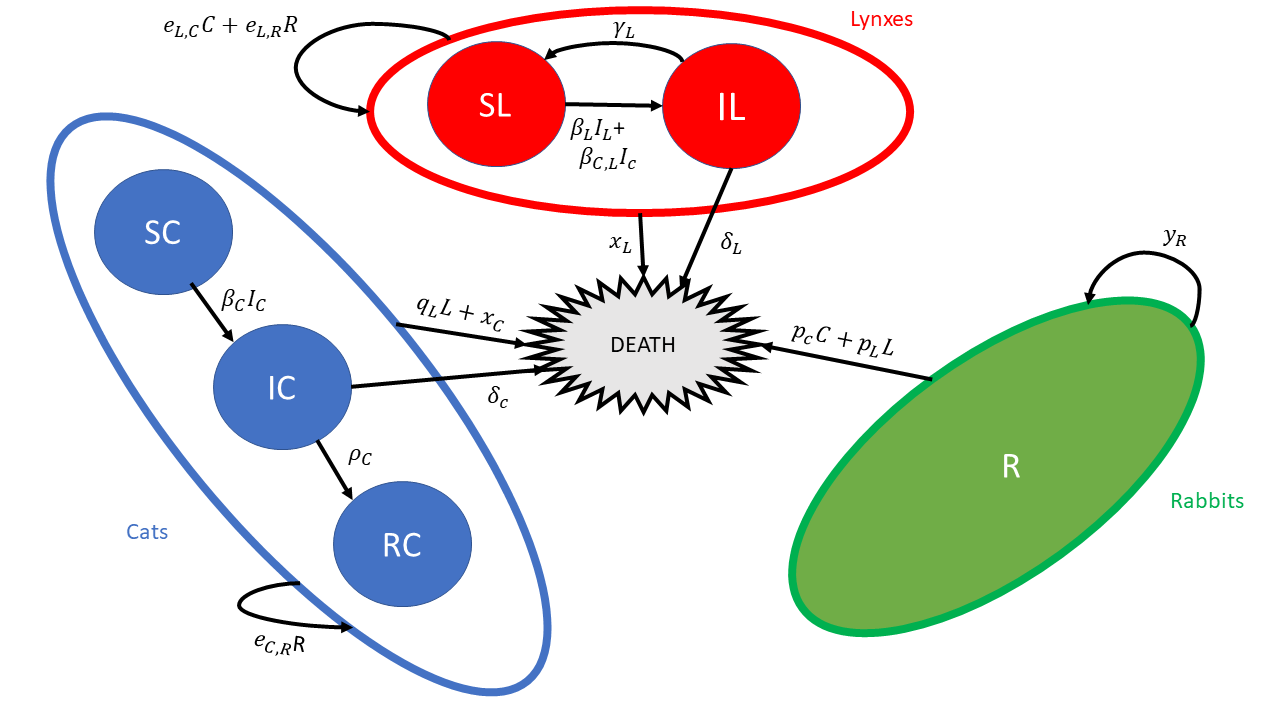
\includegraphics[scale=0.8]{images/graph.png}

Interpretation:
\begin{multicols}{2}
    $\alpha$ = contact rates between populations\\
    $\epsilon$ = fraction of cats eaten by lynxes\\
    $\beta$ = infection rates among and between population\\
    $\gamma$ = non-immunizing recovery rate \\
    $\rho$ = immunizing recovery rate\\
    $q, p$ = death by predation rates\\
    $x$ = death by starvation rates for predators\\
    $y$ = breeding rate for prey\\
    $\rightarrow$ = becomes .../increases the number of ...\\
    $\Leftrightarrow$ = in contact with ...
\end{multicols}
\quad Since the disease is assumed to be non-immunizing for lynxes, but with possible recovery, there is no Recovered compartment for lynxes. If they recover, they go back to Susceptibles. Since a lynx meeting a cat can either kill or eat it with a very small probability, we have this term $\epsilon$. For now, we assume that cats and lynxes have the same behaviour whether they are infected or not (while an infected animal may be less efficient when hunting). This is assumed for simplicity but can be improved later if desired, it depends on the symptoms of the disease. Combining all this, we have a system of 6 differential equations:
\begin{itemize}
	\item $\frac{dS_{L}}{dt} = [\alpha_{L,C}\epsilon CS_{L} + \alpha_{L,R}RS_{L} + \gamma_{L}I_{L}] - [x_{L}S_{L} + \beta_{L}I_{L}S_{L} + \beta_{C,L}\alpha_{L,C}I_{C}S_{L}]$
	\item $\frac{dI_{L}}{dt} = [\alpha_{L,C}\epsilon CI_{L} + \alpha_{L,R}RI_{L} + \beta_{L}I_{L}S_{L} + \beta_{C,L}\alpha_{L,C}I_{C}S_{L}] - [x_{L}I_{L} + \gamma_{L}I_{L} + \delta_{L}I_{L}]$
	\item $\frac{dS_{c}}{dt} = [\alpha_{C,R}RS_{C}] - [x_{C}S_{C} + q_{L} LS_{C} + \beta_{C}I_{C}S_{C}]$
	\item $\frac{dI_{C}}{dt} = [\alpha_{C,R}RI_{C} + \beta_{C}I_{C}S_{C}] - [x_{C}I_{C} + q_{L} LI_{C} + \rho_{C}I_{C} + \delta_{C}I_{C}]$
	\item $\frac{dR_{C}}{dt} = [\alpha_{C,R}RR_{C} + \rho_{C}I_{C}] - [x_{C}I_{C} + q_{L} LI_{C}]$
	\item $\frac{dR}{dt} = [y_{R}R] - [p_{C}C + p_{L}L]$
\end{itemize}	

where $L = S_{L} + I_{L}$ and $C = S_{C} + I_{C} + R_{C}$

\section{Results and Discussion}

\quad A sensitivity analysis for the parameters $\beta_L$ and $\beta_{C,L}$ will help us understand the spread of the disease. If the model is more sensitive to changes in the parameter $\beta_L$, then the lynxes are more prone to be infected due to interactions amongst lynxes on their own. On the other hand, if the model is more sensitive to $\beta_{C,L}$, then the infection spreads predominantly due to contact between the lynxes and the cats. In the former case, we could suggest conservation strategies that would isolate infected lynxes till they recover, while in the latter strategies would be to avoid lynx-cat interactions. 

\quad Further conservation strategies might be suggested based on population dynamics. If the model shows that the cats as a mesopredator might disrupt the food chain by consuming all prey rabbits before the lynx get an opportunity, then a strategy might be suggested to reduce cat-rabbit interactions. 


\printbibliography


\end{document}
